\chapter{Hardware}\label{ch:hardware}


In the following chapter the hardware used to create the robot is discussed.
The first decision made was what platform to use, based on the available resources and knowledge of use.

\section{Single board computer} 

The Raspberry Pi is the platform of choice used in the development of this project. Several factors influenced the choice, the most prominent of which was the familiarity the single board computer offered. Previous usage of Raspberry Pi 2B, allowed for faster decision making, when exploring for potential resources. 

\begin{figure}[h]
\centering
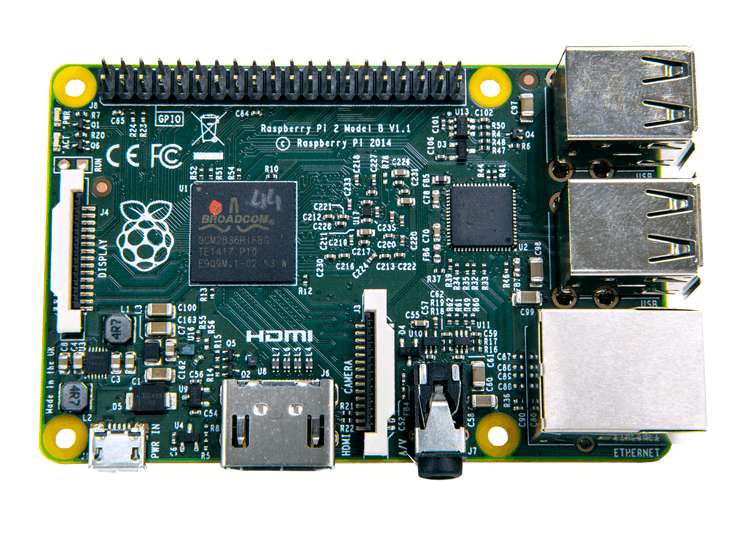
\includegraphics[width = 0.4\textwidth]{Raspberry-Pi-2}
\caption{Raspberry Pi 2B}
\label{fig::rasppi2b}
\end{figure}

\begin{figure}[h]
\centering
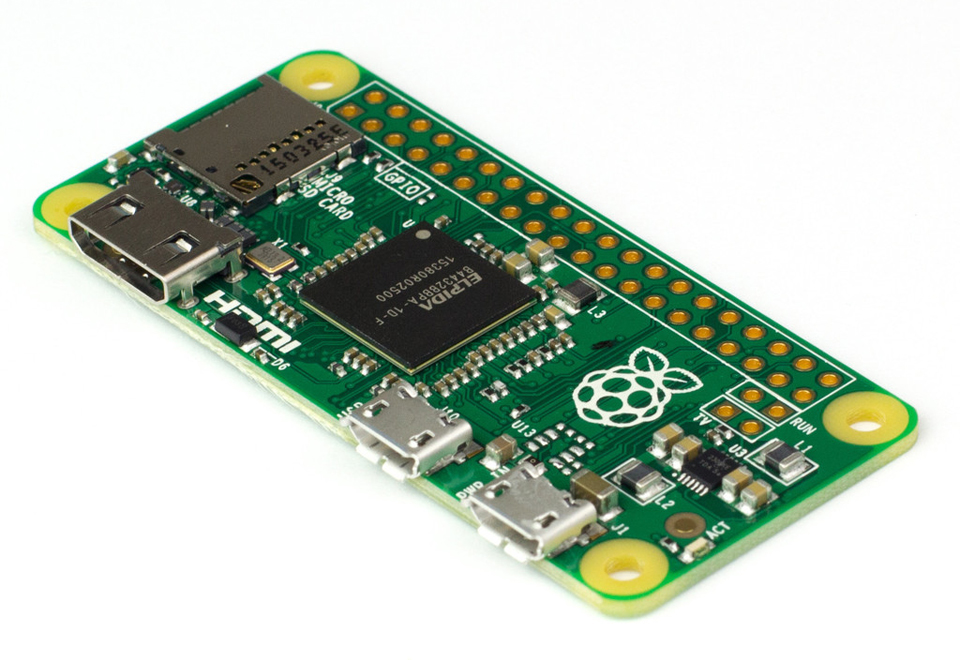
\includegraphics[width = 0.4\textwidth]{raspberry_pi_zero_1}
\caption{Raspberry Pi Zero}
\label{fig::raspizero}
\end{figure}

The initial choice was a Raspberry Pi 2B, however, after consideration of the size and required power consumption, a choice was made to use Raspberry Pi Zero instead.  

Performance of the two computers is almost similar, with the exception that the Zero model has less RAM compared to its 2B counterpart. Nevertheless, no significant impact was registered.

Specs of the Raspberry Pi Zero:
1Ghz, Single-core CPU
512MB RAM
Mini HDMI and USB On-The-Go ports
Micro USB power
HAT-compatible 40-pin header
Composite video and reset headers

\section{Distance measuring} 

Since the main purpose of the device would be to avoid obstacles, distance measuring sensors are required. There are several choices when it comes to distance sensors, vastly ranging in price and accuracy. The optimal choice would be a Lidar, however, at the time of development of this paper, the prices for Lidar were to high for practical implementation in a consumer application. 
As a result, the choice was made to use a set of ultrasonic sensors, which scaled well according to price and accuracy of measurements.
Three HC-SR04 ultrasonic sensors were used for distance measuring purposes in the device. The positioning of the sensors is on the front, and on the sides.

\begin{figure}[h]
\centering
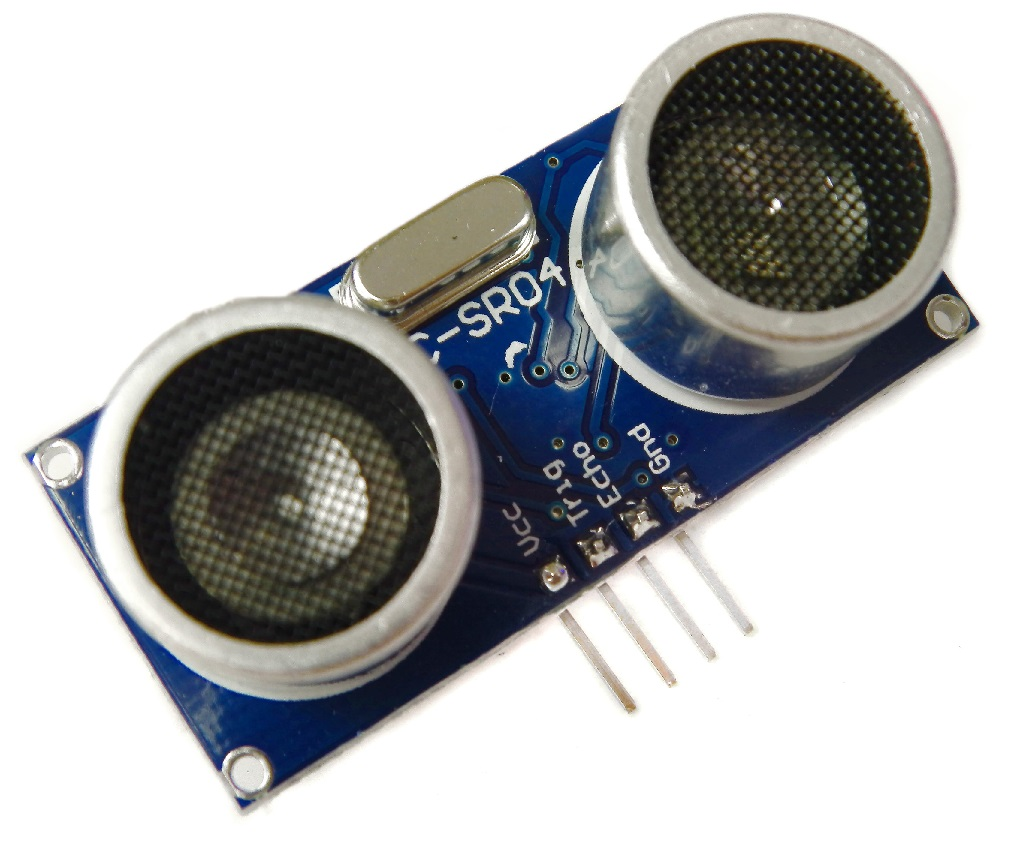
\includegraphics[width = 0.4\textwidth]{hc-sr04}
\caption{Ultra sonic sensor HC-SR04}
\label{fig::hcsr04}
\end{figure}

\section{DC motors and chassis} 

Considering the body of the robot, an inexpensive set of DC motors with a chassis was purchased and assembled. It comes with an attachable tachometer wheel for the motor, in order to incorporate a rotary encoder in the design, crucial for regulating the speed of the individual wheels.\cite{Motorref}

\begin{figure}[h]
\centering
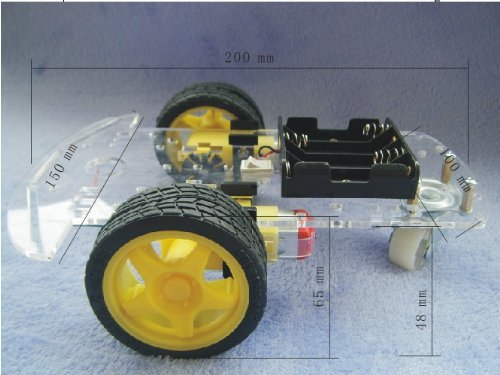
\includegraphics[width = 0.4\textwidth]{chassie}
\caption{Chassie and the two DC motors with a power supply}
\label{fig::chassie}
\end{figure}

Motor specs:

Voltage:
DC 3V
DC 5V
DC 6V
Current:
100 MA
100MA
120MA
Reduction rate:48:1
RPM (With tire):100,190,240
Tire Diameter:66mm
Car Speed(M/minute):20,39,48

Motor Weight (g):50

Motor Size:70mm*22mm*18mm

Noise:<65dB 

The two motors are identical and are used to move, as well as steer, the device and to 

\section{Motor driver} 

At the beginning of the project a L9110S DC Stepper Motor Driver H-Bridge was used, capable of controlling the direction of rotation of the wheels, but it was soon discovered the suggested driver was not capable of regulating the motor speeds.
To control the speed of the robot, a replacement with a L298N driver had to be performed.
The second driver was capable of using the PWM to regulate the speed of the motors.

\begin{figure}[h]
\centering
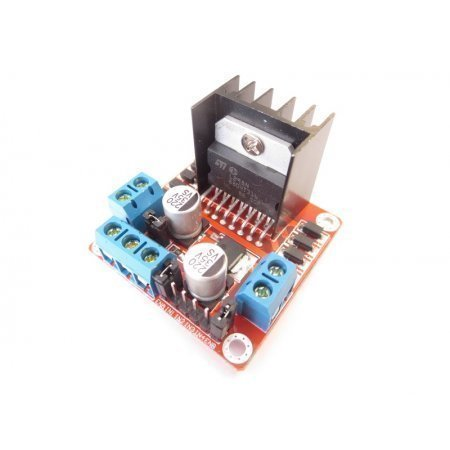
\includegraphics[width = 0.4\textwidth]{driver2}
\caption{The L298N driver}
\label{fig::driver2}
\end{figure}

Driver specs:
Working mode:	H bridge (double lines)
Control chip:	L298N (ST)
Logical voltage:	5V
Driving voltage:	5V-35V
Logical current:	max 36mA
Driving current:	2A (max single bridge)
Maximum power:	25W
Storage temperature:	-20 C +135 C
Periphery dimension:	43 x 43 x 27mm(L x W x H)

\section{Speed sensor}

The speed of the wheels is measured by the LM393 IR speed sensors attached to the tachometer wheel of the motor.\cite{SpeedSensor}

\begin{figure}[h]
\centering
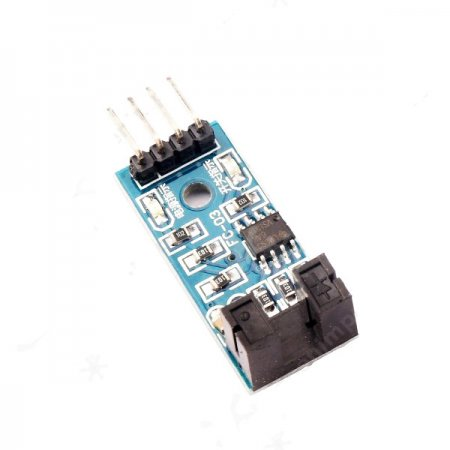
\includegraphics[width = 0.4\textwidth]{irspeed}
\caption{The LM393 IR speed sensor}
\label{fig::driver2}
\end{figure}

The speed sensor is used to estimate the error of the wheel speed.
Features:

Working voltage: 3.3V~5V
Weight: 8g
Dimensions: Approx.3.2 x 1.4 x 0.7cm
5mm Groove width
Using wide voltage LM393 comparator
Application: Widely used in dynamo speed detecting, pulse counting, etc
Output form: Digital switch output (0 and 1) and Analog for Sensitivity.


\section{Wi-Fi adapter}

In order to perform wireless monitoring, as well as extend the connectivity, an Edimax EW-7811Un Wi-Fi adapter, was used. 

\begin{figure}[h]
\centering
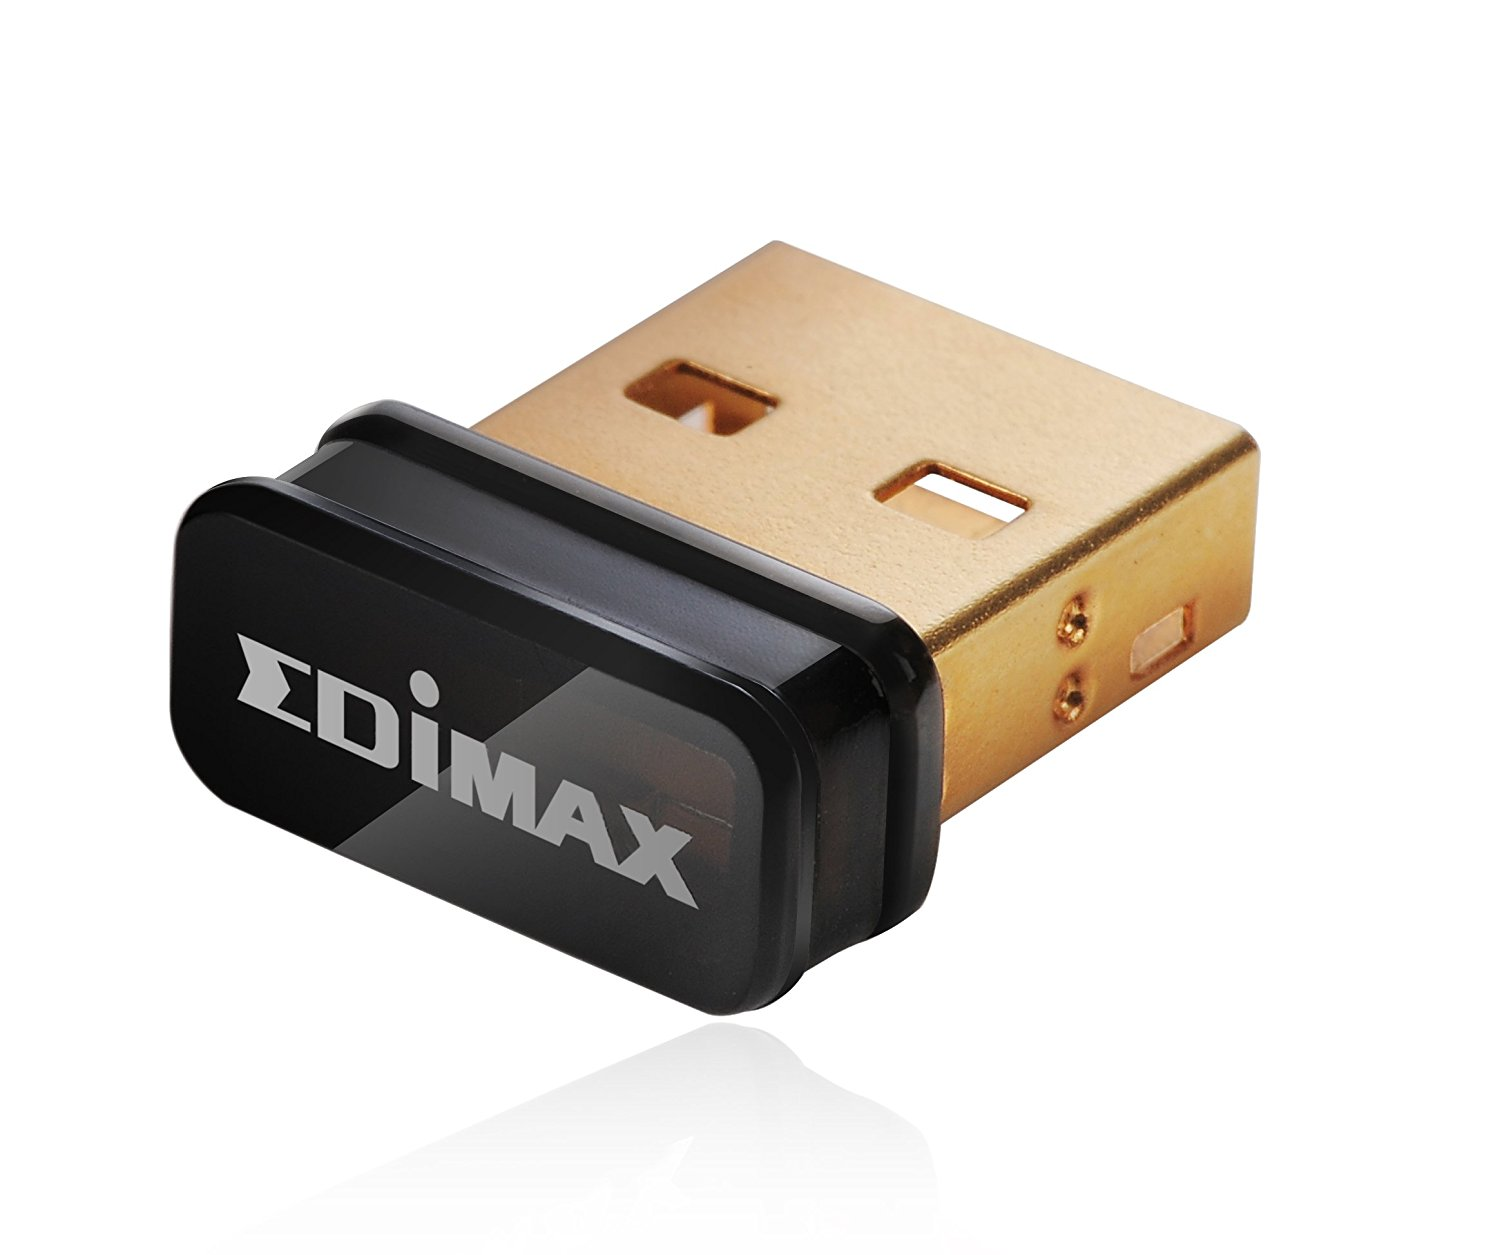
\includegraphics[width = 0.4\textwidth]{edimax}
\caption{Edimax EW-7811Un Wi-Fi adapter}
\label{fig::edimax}
\end{figure}

\section{Assembly}

In this section, the schematics of the assembled components has been analysed and given in figure \ref{fig::schematics}.

\begin{figure}[h] 
\centering
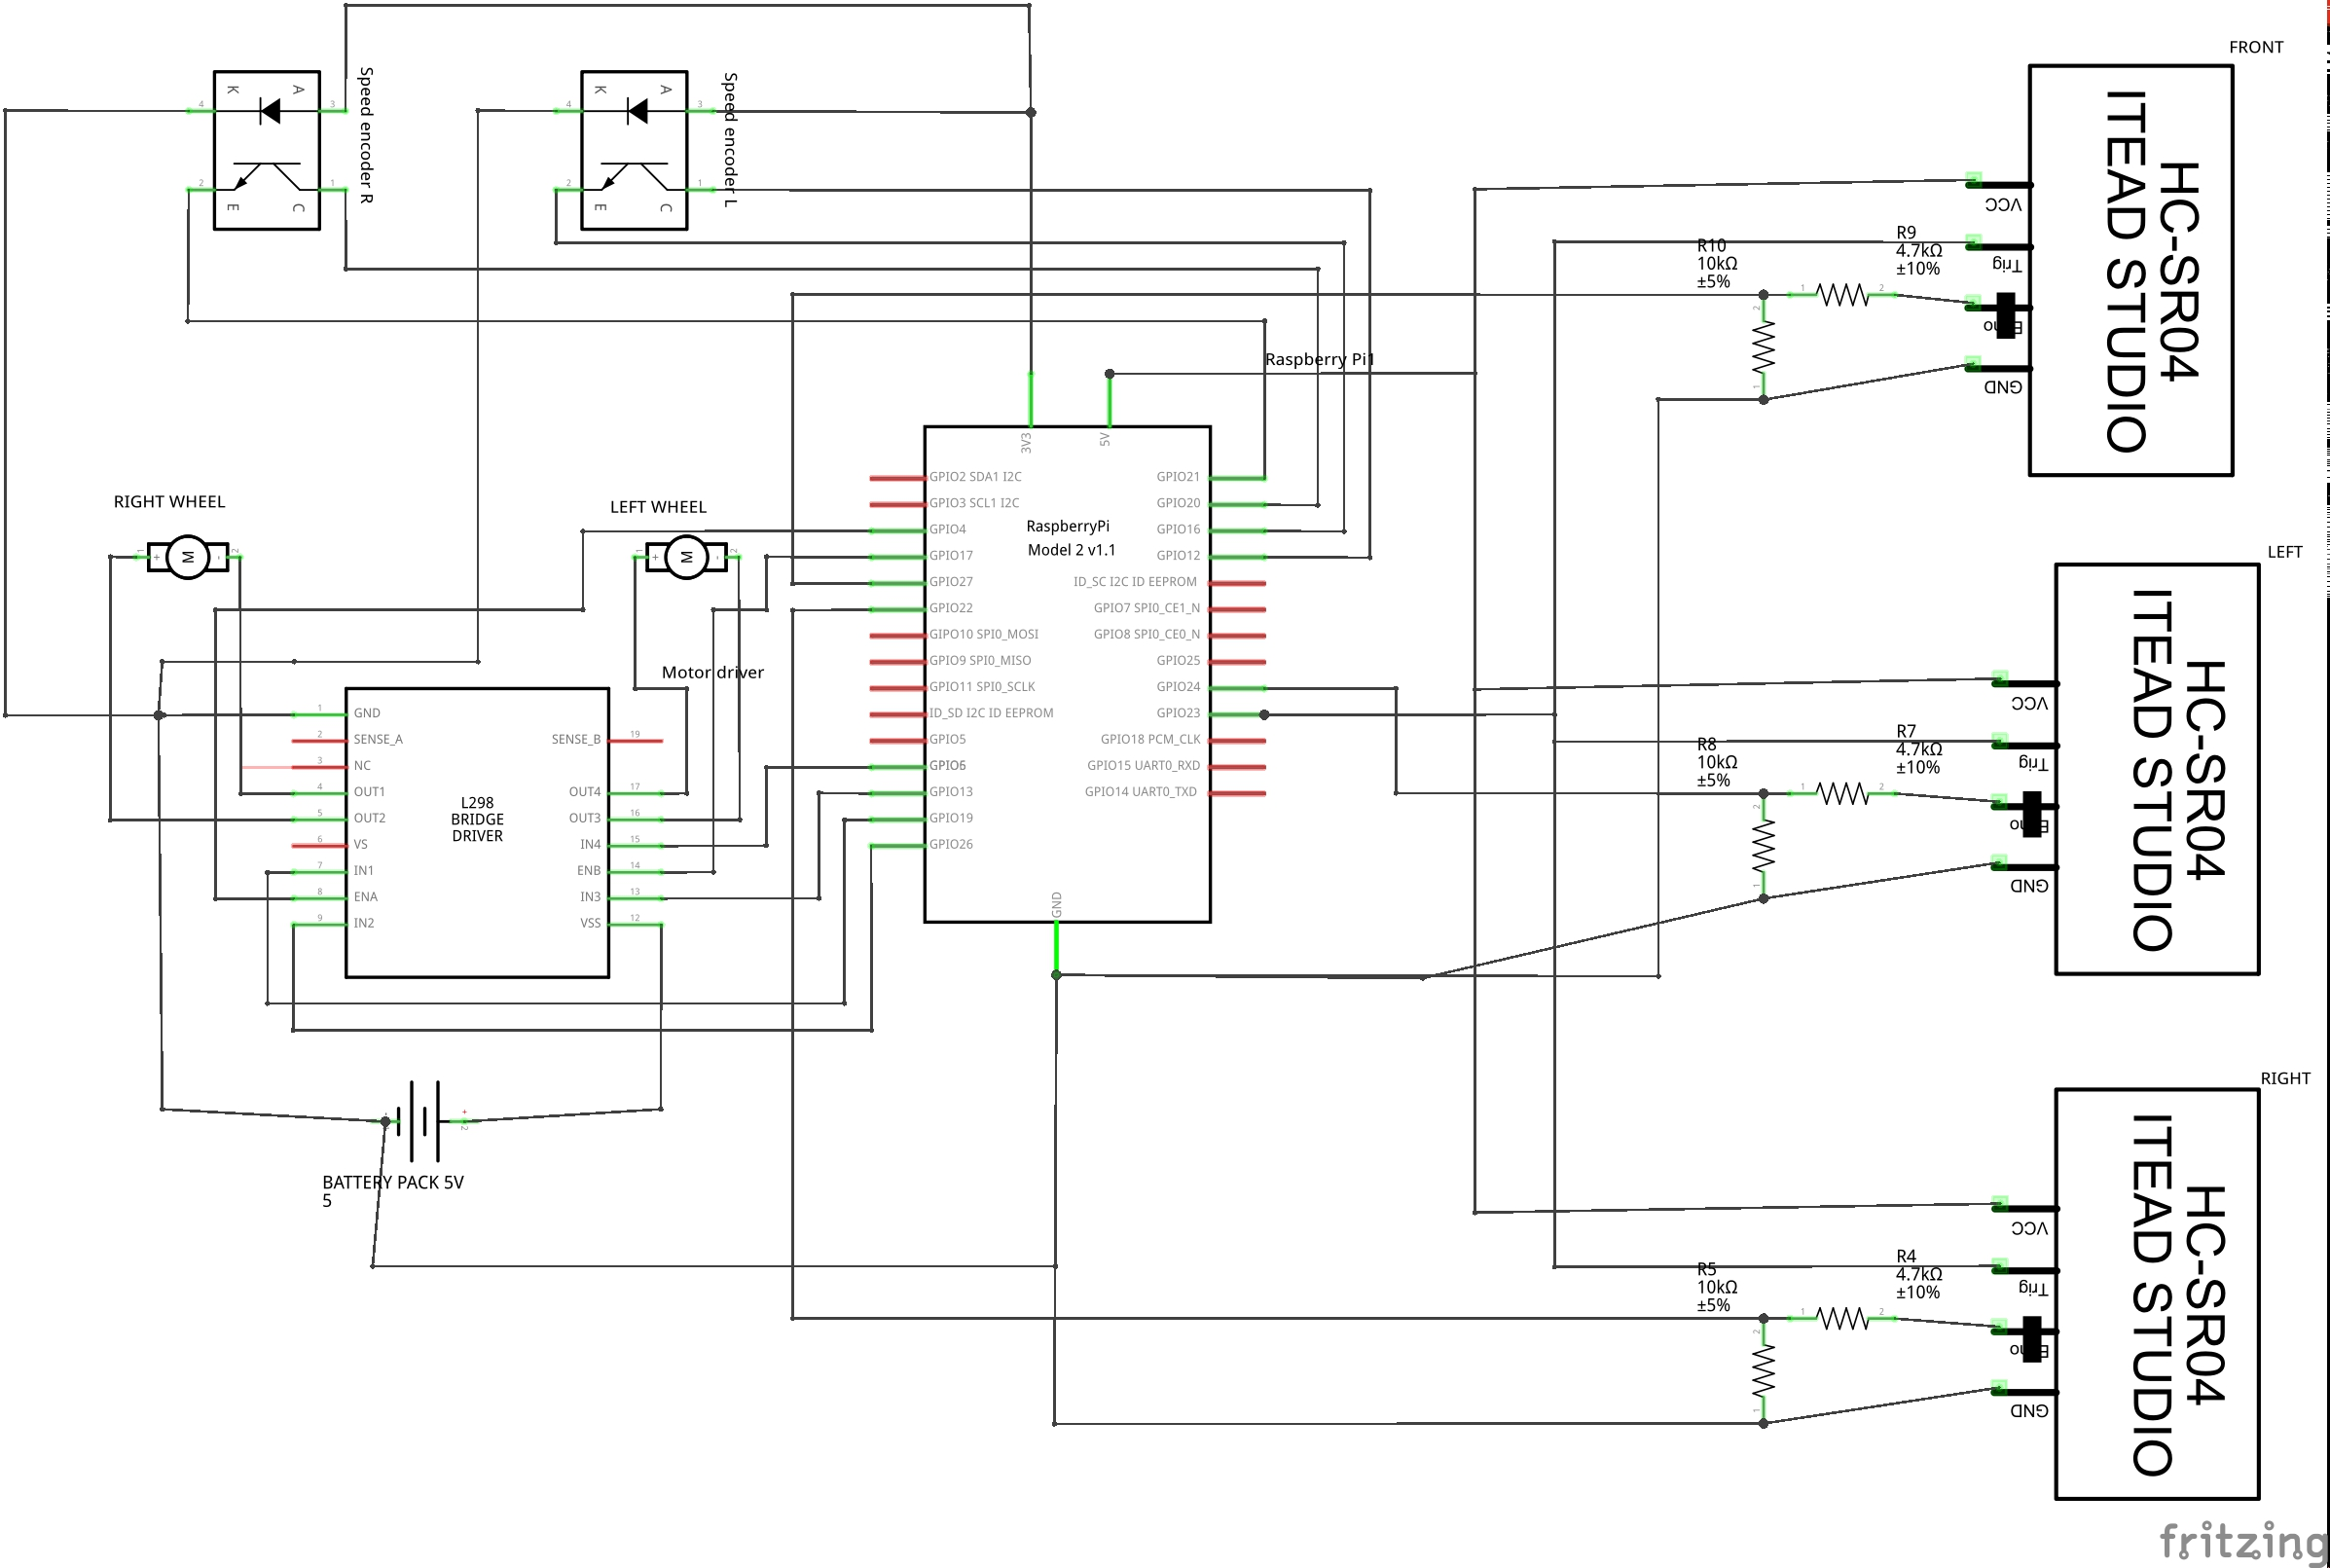
\includegraphics[width = 1\textwidth]{P51_schem}
\caption{Schematics of the device}
\label{fig::schematics}
\end{figure}

In the middle section of the schematics, the Raspberry Pi is present. Unfortunately, the software used to make this schematic did not have the Raspberry Pi Zero layout, so the model 2 was used instead. Regarding the project there is not a big difference, as the pins are the same as Zero.

On the right side of the system three ultrasonic sensors could be seen, connected to the Raspberry Pi. The Vcc and GND pins are all connected to the Raspberry, allowing the sensors to draw power from the microcontroller itself. The trigger pins are all connected to the same Raspberry pin, meaning that when one of the sensors is triggered all of them will emit sonic impulse.
The triggers are all on the same pin to not limit the number of available pins on the Raspberry. However there is not a significant difference,as the echo pins of each of the sensors go into separate ports on the Raspberry and each of them has a voltage divider connected to the GND.

The driver is present in the bottom left of the schematics, alongside a battery pack connected to the driver and providing power to both motors. It is connected to the Raspberry by six pins, four responsible for the direction of the motors(2 for each motor) and 2 enable pins, used for controlling the speed of the motor by PWM.

\newpage
The motors are connected directly to the driver, by two wires.
The two encoders, responsible for monitoring the speed of the wheels, are present in the top left of the schematics
An external power source was used for the Raspberry Pi, which is not present in this schematics.


